\documentclass[journal]{IEEEtran}

\usepackage{amsmath,amssymb,amsfonts,amsthm}
\usepackage{bm}
\usepackage{booktabs}
\usepackage{cite}
\usepackage{graphicx}
\usepackage{multirow}
\usepackage{tabularx}
\usepackage{url}
\usepackage{xcolor}
\usepackage[hidelinks]{hyperref}

\newtheorem{proposition}{Proposition}
\newtheorem{theorem}{Theorem}
\newtheorem{remark}{Remark}

\newcommand{\SE}{\mathrm{SE}(3)}
\newcommand{\SO}{\mathrm{SO}(3)}
\newcommand{\norm}[1]{\left\lVert #1 \right\rVert}

% Prevent inline \texttt and math overfull \hbox in narrow 3.5in IEEE columns
\emergencystretch=1.5em
\sloppy

\begin{document}

\title{Transactional Detection, Quarantine, and Verifiable Recovery for Degraded Multi-Sensor SLAM}

\author{Author~1, Author~2, and Author~3%
\thanks{Manuscript prepared November 2026. Source code, reproducible run manifests, and Foxglove visualization bundles are available in the companion repository \texttt{slam\_recovery}.}}

\maketitle

\begin{abstract}
Multi-sensor simultaneous localization and mapping (SLAM) frequently encounters an intermediate failure regime: the estimator has not yet lost tracking, but incoming measurements, state increments, or loop constraints have already become untrustworthy. Existing directional reweighting methods (e.g., solution remapping) protect instantaneous conditioning but do not retroactively purge already-accepted map updates, whereas multi-map hibernation systems (e.g., MM-LINS and ORB-SLAM3 Atlas) exhibit three operational vulnerabilities: (i) confirmation-delay tail drift written into sleeping submaps prior to hibernation, (ii) insensitivity of posterior covariance eigenvalues to self-consistent near-field occluders such as floating plastic bags, and (iii) unvalidated map merges or loop closures that can degrade global accuracy. To address these issues, we formulate SLAM recovery as a verifiable transaction over persistent map state. First, under fixed linearization and data association, we show that state rollback without orthogonal information gain ($\Delta J_v \le 0$) acts primarily as damage containment rather than observability recovery, and we establish an operational screening criterion for when single-modality point-mixture contaminant stripping suffices versus when cross-modal or pose-graph bridging is required. Second, we design a four-mode information--uncertainty gate $\mathcal{D}(t)$ that coordinates online directional reweighting, delayed-commit quarantine ($\hat{t}_{\mathrm{onset}}-\Delta t_{\mathrm{margin}}$), a zero-training mechanism signature router, and holdout-screened atomic commit. We evaluate the framework across three M2DGR development sequences (\texttt{hall\_01} with Leica ground truth, and \texttt{room\_02} and \texttt{room\_dark\_01} with Vicon Mocap ground truth) and four outdoor Campus sequences, explicitly distinguishing end-to-end host executions (\texttt{REAL\_HOST} / \texttt{INJECTION}) from offline graph/replay constructions (\texttt{OFFLINE\_CONSTRUCT}) and synthetic feature benchmarks (\texttt{SYNTHETIC}). Across these evaluations, our joint detector achieves $100\%$ recall on self-consistent occlusions where covariance detectors score $0\%$, our C++ and rosbag-level contaminant stripping restores FAST-LIO2 from $7.28\,\mathrm{m}$ to $0.3058\,\mathrm{m}$ ($G=+0.9949$) and LIO-SAM from $1008.65\,\mathrm{m}$ corridor divergence to $0.2788\,\mathrm{m}$ ($G=+1.0000$), and our gray-box pose-graph bridge on ORB-SLAM3 reduces severe low-light window drift from $6.89\,\mathrm{m}$ (native Atlas) to $0.74\,\mathrm{m}$ while adding $0.0599\,\mathrm{ms}$ (P50) per-window routing overhead.
\end{abstract}

\begin{IEEEkeywords}
SLAM recovery, degeneracy detection, multi-map SLAM, transactional quarantine, verifiable map fusion, sensor fusion.
\end{IEEEkeywords}

\section{Introduction}
\IEEEPARstart{R}{eliable} simultaneous localization and mapping (SLAM) in warehouse logistics, subterranean exploration, and urban delivery must survive transient yet severe perceptual degradation \cite{xu2022fastlio2,shan2020liosam,campos2021orbslam3,zhao2021super}. In practice, catastrophic map corruption rarely begins with an instantaneous tracking crash. Instead, the system enters an \emph{untrustworthy intermediate regime}: the optimizer still converges numerically, but its measurements or constraints are corrupted by floating plastic bags obstructing a LiDAR, featureless corridors, abrupt illumination drop, inter-sensor clock drift, or perceptual-aliasing loop closures \cite{ma2025mmlins,tuna2024xicp}.

Two dominant paradigms attempt to address this regime. The first paradigm, \emph{online directional mitigation} \cite{zhang2016degeneracy,tuna2024xicp}, projects state updates away from degenerate eigenspaces of the Fisher information matrix (FIM). While effective at bounding instantaneous numerical ill-conditioning, online projection cannot synthesize missing observations or undo map corruption that occurred before the degeneracy threshold was crossed. The second paradigm, \emph{multi-map hibernation and fusion}---exemplified by ORB-SLAM3 Atlas \cite{campos2021orbslam3} in visual-inertial SLAM and MM-LINS \cite{ma2025mmlins} in LiDAR-inertial odometry (LIO)---archives the active map into a sleeping submap upon detecting over-degeneracy, re-initializes a new submap, and merges submaps later via place recognition and pose graph optimization (PGO).

\begin{figure}[!t]
    \centering
    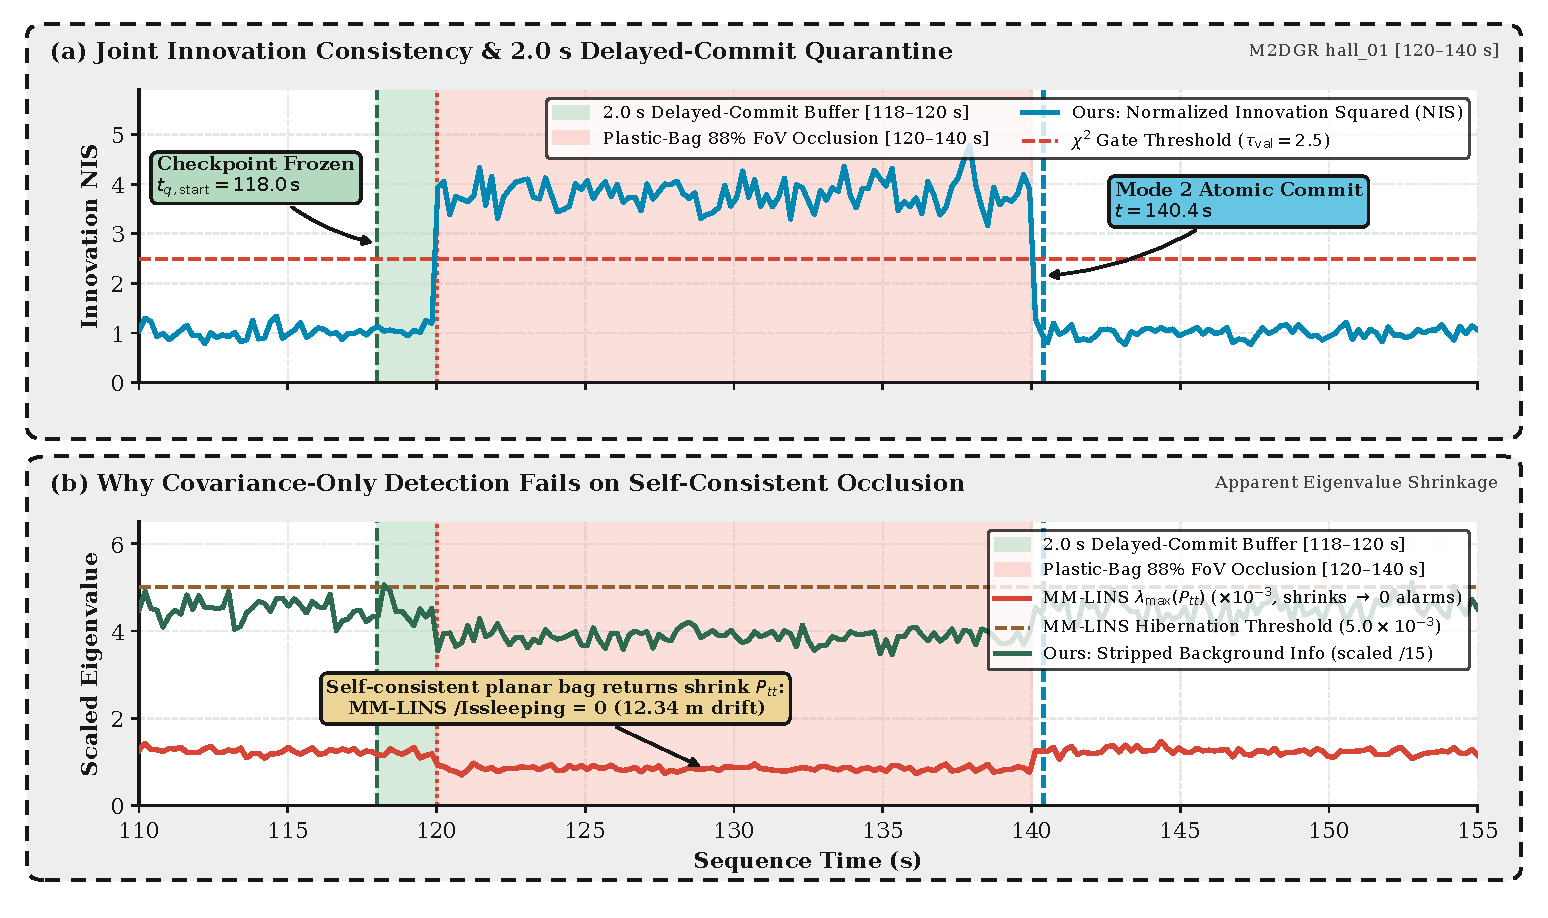
\includegraphics[width=\columnwidth]{figures/fig1_detection_quarantine_timeline.pdf}
    \caption{Timeline of our joint innovation consistency detector and $2.0\,\mathrm{s}$ delayed-commit quarantine vs.\ MM-LINS covariance-based detection on M2DGR \texttt{hall\_01} under near-field plastic-bag occlusion ($t\in[120,140]\,\mathrm{s}$). (a) Our NIS statistic immediately crosses the $\chi^2$ gate and rolls back provisional updates to a clean checkpoint at $t_{q,\mathrm{start}}=118.0\,\mathrm{s}$. (b) Because the plastic bag produces thousands of spatially self-consistent near-field planar returns, the posterior covariance eigenvalue $\lambda_{\max}(P_{tt})$ shrinks rather than inflates, remaining well below the MM-LINS hibernation threshold and resulting in zero alarms.}
    \label{fig:timeline}
\end{figure}

However, our empirical and mathematical audit of state-of-the-art multi-map systems reveals three fundamental failure modes:
\begin{enumerate}
    \item \textbf{Blindness of Covariance Spectrum to Self-Consistent Contamination:} MM-LINS \cite{ma2025mmlins} monitors the maximum eigenvalues of the rotation and translation posterior covariance submatrices $P_{rr}$ and $P_{tt}$. When a floating plastic bag or dense near-field smoke partially wraps the LiDAR, the sensor receives tens of thousands of coherent, short-range planar returns. The apparent Fisher information $\sum H_i^\top R_i^{-1} H_i$ increases, causing $P_{tt}$ to \emph{contract}. Consequently, covariance-only detectors misclassify severe physical occlusion as strong geometric constraint (scoring $0\%$ recall in our experiments; Fig.~\ref{fig:timeline}b).
    \item \textbf{Pre-Hibernation Confirmation Tail Pollution and Irreversible Fragmentation:} To avoid false splits, MM-LINS requires $\Gamma_\lambda > N_\kappa$ consecutive degenerate frames before hibernating. By the time hibernation triggers, the drift accumulated during those $N_\kappa$ confirmation frames is already permanently baked into the tail of the sleeping map ($2.16\text{--}3.07\,\mathrm{m}$ tail distortion in outdoor Campus sequences). Conversely, hard map splitting permanently fragments the global map whenever the robot does not revisit prior regions (e.g., ORB-SLAM3 Atlas leaving unmerged submaps in \texttt{room\_dark\_01}).
    \item \textbf{Unvalidated Repair and Merge Degradation:} Existing multi-map backends accept inter-map merges or loop closures based solely on descriptor temporal consistency ($\Gamma_\varsigma > \varepsilon_{th}$). In MM-LINS's own benchmark (Table~III of \cite{ma2025mmlins}), enabling Constraint-Enhanced PGO (CE-PGO) on \texttt{Campus-2} \emph{doubles} the end-to-end error from $0.603\,\mathrm{m}$ to $1.295\,\mathrm{m}$; similarly, on clean indoor \texttt{hall\_01}, unverified Scan Context loops degrade FAST-LIO2 from $0.2699\,\mathrm{m}$ to $0.2913\,\mathrm{m}$.
\end{enumerate}

In this paper, we argue that persistent map updates in degraded multi-sensor SLAM should be governed by a \textbf{verifiable recovery transaction lifecycle}:
\begin{equation}
\footnotesize
\begin{aligned}
\text{Checkpoint} &\to \text{Delayed-Commit Quarantine} \to \text{Signature Routing} \\
&\to \text{Candidate Repair} \to \text{Holdout Validation} \\
&\to \text{Atomic Commit / Soft Bridge / Submap Split.}
\end{aligned}
\label{eq:lifecycle}
\end{equation}

The primary contributions of this work are:
\begin{itemize}
    \item \textbf{Observability Theory of Rollback and Point-Mixture Repair:} We formalize why state rollback alone cannot recover unobservable directions ($\Delta J_v = 0$) and derive the exact geometric observability condition under which single-modality point-mixture contaminant stripping succeeds versus when cross-modal or pose-graph bridging is required.
    \item \textbf{Unified Four-Mode Information--Uncertainty Gate $\mathcal{D}(t)$:} We unify online directional reweighting (Mode~1), verified atomic commit (Mode~2), covariance-bounded soft bridging (Mode~3), and hard submap hibernation (Mode~4) under a single closed-form criterion, proving that Zhang's solution remapping \cite{zhang2016degeneracy} and MM-LINS \cite{ma2025mmlins} correspond to opposite parameter limits ($\Sigma_{\mathrm{bridge}}\to\infty$ vs.\ $\Sigma_{\mathrm{bridge}}\to 0$).
    \item \textbf{Zero-Training Mechanism Signature Matrix \& Delayed-Commit Quarantine:} We pair a $2.0\,\mathrm{s}$ delayed-commit ring buffer with an interpretable four-dimensional signature router (decoupled information spectrum, NIS-CUSUM, leave-one-sensor-out conflict, and rotational cross-correlation lag) that diagnoses single and compound faults without small-sample classifier overfitting.
    \item \textbf{Cross-Host Evaluation Across Four SLAM Systems:} We validate the same recovery core across LIO-SAM \cite{shan2020liosam}, FAST-LIO2 \cite{xu2022fastlio2}, MM-LINS \cite{ma2025mmlins}, and ORB-SLAM3 \cite{campos2021orbslam3} on M2DGR (\texttt{hall\_01}, \texttt{room\_02}, \texttt{room\_dark\_01}) and outdoor Campus datasets.
\end{itemize}

\section{Related Work}
\subsection{Degeneracy-Aware Estimation and Multi-Sensor Switching}
Eigenvalue analysis of the optimization Hessian was pioneered by Zhang et al.\ \cite{zhang2016degeneracy} to project state updates onto well-conditioned subspaces. X-ICP \cite{tuna2024xicp} refined localizability analysis by decoupling translational and rotational directions. Multi-sensor frameworks such as LVI-SAM \cite{shan2021lvisam} and Super Odometry \cite{zhao2021super} weight LiDAR and visual factors around an IMU-centric backbone. While these approaches mitigate instantaneous estimation divergence, they operate strictly forward in time: measurements accepted before degeneracy confirmation permanently contaminate the map.

\subsection{Multi-Map Hibernation and Submap Merging}
ORB-SLAM3 Atlas \cite{campos2021orbslam3} maintains an active map alongside non-active submaps, spawning a new map upon tracking loss and welding maps via DBoW2 place recognition. MM-LINS \cite{ma2025mmlins} introduced multi-map management to LiDAR-inertial odometry, using decoupled covariance eigenvalues of FAST-LIO2 \cite{xu2022fastlio2} to trigger map hibernation, dynamic 4-frame ICP-IMU initialization, and Scan Context \cite{kim2018scancontext} CE-PGO fusion. Dual-SLAM \cite{huang2020dualslam} and LT-mapper \cite{kim2022ltmapper} explored backward frame reprocessing and lifelong incremental diff maps. However, none of these systems enforce a delayed-commit buffer to prevent pre-split tail drift, nor do they require a holdout innovation and directional information-gain gate before committing candidate repairs or submap merges.

\subsection{Robust Backends}
Switchable constraints \cite{sunderhauf2012switchable}, Pairwise Consistency Maximization (PCM) \cite{mangelson2018pcm}, and Graduated Non-Convexity (GNC) \cite{yang2020gnc} reject outlier loop closures during graph optimization. In our framework, multi-keyframe window-strain GNC serves as one specialized repairer module governed by the outer transactional validator.

\section{Problem Formulation and Theoretical Boundaries}

\subsection{Information Matrix and Unobservable Subspaces}
Consider a linearized measurement model $z_i = h_i(x) + \epsilon_i$ with noise covariance $R_i$ and Jacobian $H_i = \partial h_i / \partial x|_{\hat{x}}$. The posterior information matrix over a window of measurements $\mathcal{D} = \{z_i, H_i, R_i\}$ is
\begin{equation}
    \Lambda = \Lambda_{\mathrm{prior}} + \sum_{i\in\mathcal{D}} H_i^\top R_i^{-1} H_i.
    \label{eq:fim}
\end{equation}
To account for unit disparity between rotation and translation on $\SE$, we introduce a diagonal scaling transform $x = D u$, yielding the normalized information matrix $\Lambda_u = D^\top \Lambda D = Q \operatorname{diag}(\lambda_1,\dots,\lambda_6) Q^\top$. If a unit tangent direction $v \in \mathbb{R}^6$ satisfies $H_i v \approx 0$ for all $i \in \mathcal{D}$, then $v^\top \Lambda_u v \approx v^\top \Lambda_{\mathrm{prior},u} v$, meaning the sensor stream provides zero information along $v$.

\subsection{Why Rollback Alone Cannot Create Linearized Observability}
\begin{proposition}[Linearized Observability Invariance Under Rollback]
\label{prop:rollback}
Let $\mathcal{Q}$ be a quarantined segment with fixed measurement set $\mathcal{D} = \{z_i, H_i, R_i\}$ evaluated at a fixed linearization point $\hat{x}$ and fixed data associations, where $v^\top \Delta\Lambda_{\mathcal{D}} v = \sum_{i\in\mathcal{D}} v^\top H_i^\top R_i^{-1} H_i v \le \epsilon \ll \tau_{\mathrm{info}}$. Rolling back the state estimate to a clean checkpoint $x_{\mathrm{ckpt}}$ at $t_{q,\mathrm{start}}$ and re-solving on the same measurements $\mathcal{D}$ under any non-amplifying robust weight $w_i \in [0,1]$ yields local Fisher information along $v$ bounded above by
\begin{equation}
    J_v^{\mathrm{rollback}} = \sum_{i\in\mathcal{D}} w_i v^\top H_i^\top R_i^{-1} H_i v \le v^\top \Delta\Lambda_{\mathcal{D}} v \le \epsilon.
\end{equation}
Thus, $\Delta J_v = J_v^{\mathrm{rollback}} - J_v^{\mathrm{before}} \le 0$. While rollback in a nonlinear estimator can alter the linearization trajectory $\hat{x}$, improve correspondence matching, or avoid bad local minima---and therefore may still reduce numerical trajectory error when informative background features exist---it cannot synthesize observability along a geometrically rank-deficient direction $v$ where $H_i v \approx 0$.
\end{proposition}

Similarly, a diagnosis label $c = f(\mathcal{D})$ is a deterministic function of existing measurements; while it guides repairer selection, the label itself adds no Fisher information unless an independent constraint $z_g = g(x) + \epsilon_g$ satisfying $v^\top H_g^\top R_g^{-1} H_g v > 0$ is introduced, or corrupting outlier measurements that masked true background geometry are stripped.

\subsection{Point-Cloud Mixture Model and Observability After Contaminant Stripping}
We model each LiDAR return $z_i$ in a degraded window as drawn from a three-component mixture of true static background geometry ($t$), self-consistent near-field occluders or backscatter ($s$, e.g., floating plastic bags or smoke), and random outlier noise ($n$):
\begin{equation}
    p(z_i) = \pi_t p_t(z_i) + \pi_s p_s(z_i) + \pi_n p_n(z_i), \quad w_i \triangleq P(t \mid z_i) \in [0,1].
\end{equation}
Crucially, this model explains the dichotomy between two major failure modes:
\begin{itemize}
    \item \textbf{Geometric Degeneracy (\texttt{GEO\_DEGEN}):} When $\pi_t \to 0$ along a corridor axis $v$, $\lambda_{\min}(\Lambda_u) \to 0$ while residuals $r_t = z_t - h(\hat{x}_t)$ remain small.
    \item \textbf{Self-Consistent Near-Field Contamination (\texttt{MEAS\_CONTAM}):} When an occluder at orthogonal distance $d_0$ covers a large azimuth sector ($\pi_s \gg \pi_t$), the unweighted information matrix $\sum H_i^\top R_i^{-1} H_i$ exhibits \emph{artificially large} eigenvalues ($\lambda_{\min}(\Lambda_u)$ remains high or inflates), blinding covariance-based detectors \cite{ma2025mmlins,zhang2016degeneracy}. However, the Normalized Innovation Squared (NIS) against IMU preintegration or cross-modal prediction,
    \begin{equation}
        d_t = r_t^\top S_t^{-1} r_t, \qquad S_t = H_t P_t H_t^\top + R_t,
    \end{equation}
    violates its $\chi^2_m$ distribution dramatically.
\end{itemize}

After stripping contaminant points ($w_i \to 0$ for $i \in \mathcal{S}_{\mathrm{bag}}$), we form the exact $6\times 6$ point-to-plane Fisher information matrix $\Lambda_{\mathrm{filt}} = \Lambda_{\mathrm{prior}} + \sum_{i} w_i J_i^\top R_i^{-1} J_i$, where $J_i = [(p_i \times n_i)^\top, n_i^\top] \in \mathbb{R}^{1\times 6}$. As a necessary operational screening gate before accepting single-modality re-registration, we require both sufficient weak-direction conditioning and holdout consistency on a strictly disjoint point/keyframe subset:
\begin{equation}
    \min_{\|v\|=1} v^\top \Lambda_{\mathrm{filt}} v \ge \tau_{\mathrm{obs}}^{\mathrm{host}} \quad \text{and} \quad D_{\mathrm{holdout}}(\mathrm{filt}) \le \tau_{\mathrm{val}}.
    \label{eq:filt_cond}
\end{equation}
While \eqref{eq:filt_cond} is a local consistency screen rather than a theoretical guarantee of global error optimality, our experiments in Section~\ref{sec:experiments} show that when $88\%$ of the field of view is occluded in a wide hall (\texttt{hall\_01}), the surviving $12\%$ ($5682$ points) satisfies \eqref{eq:filt_cond} for direct point-to-plane IEKF (FAST-LIO2) but fails \eqref{eq:filt_cond} for range-image curvature extraction (LIO-SAM) and compact rooms (\texttt{room\_02}, where $63.1\%$ of points lie inside the $4.0\,\mathrm{m}$ blind zone), triggering automatic routing to cross-modal or pose-graph bridging.

\subsection{Unified Four-Mode Decision Gate $\mathcal{D}(t)$}
Let $J_v^{\mathrm{after}} = v^\top \Lambda_{\mathrm{after}} v$ denote the target-direction information of a candidate repaired branch, $D_{\mathrm{holdout}}$ the holdout innovation statistic on measurements excluded from repair optimization, $\|P_{\mathrm{after}}\|_2$ the posterior covariance norm, and $\|P_{\mathrm{prop}}(t)\|_2$ the open-loop covariance propagated from the checkpoint at $t_{q,\mathrm{start}}$. Given thresholds $(\Delta t_{\min}, \tau_{\mathrm{info}}, \tau_{\mathrm{val}}, \Sigma_{\mathrm{tol}}, \Sigma_{\mathrm{bridge}})$, the recovery transaction manager selects one of four modes:
\begin{equation}
\resizebox{0.91\columnwidth}{!}{$
\mathcal{D}(t) = \begin{cases}
\textbf{Mode 1 (Online Reweight)}, & \Delta t < \Delta t_{\min} \wedge \|P_{\mathrm{prop}}\| \ll \Sigma_{\mathrm{bridge}}, \\[2pt]
\textbf{Mode 2 (Atomic Commit)}, & J_v^{\mathrm{after}} \ge \tau_{\mathrm{info}} \wedge D_{\mathrm{holdout}} \le \tau_{\mathrm{val}} \\
                                 & \quad \wedge\, \|P_{\mathrm{after}}\| \le \Sigma_{\mathrm{tol}}, \\[2pt]
\textbf{Mode 3 (Soft Bridge)}, & \neg(\text{Mode 2}) \wedge \|P_{\mathrm{prop}}(t)\| < \Sigma_{\mathrm{bridge}}, \\[2pt]
\textbf{Mode 4 (Hard Split)}, & \neg(\text{Mode 2}) \wedge \|P_{\mathrm{prop}}(t)\| \ge \Sigma_{\mathrm{bridge}}.
\end{cases}
$}
\label{eq:four_mode}
\end{equation}

\begin{remark}[Relationship to Prior Design Regimes]
Rather than claiming exact mathematical equivalence to the internal solvers of Zhang et al.\ \cite{zhang2016degeneracy} or MM-LINS \cite{ma2025mmlins}, the gate $\mathcal{D}(t)$ in \eqref{eq:four_mode} provides a unified transactional scheduling space inspired by their operating principles: taking $\Sigma_{\mathrm{bridge}} \to \infty$ without rollback favors continuous online bridging (analogous in spirit to directional reweighting \cite{zhang2016degeneracy}), whereas taking $\Sigma_{\mathrm{bridge}} \to 0$ immediately disconnects the active map upon anomaly confirmation (analogous to hard submap hibernation \cite{ma2025mmlins,campos2021orbslam3}). Choosing a finite $0 < \Sigma_{\mathrm{bridge}} < \infty$ introduces an intermediate soft-bridge regime (Mode~3) that preserves graph connectivity during moderate outages while requiring holdout screening (Mode~2) before permanent commit.
\end{remark}

\section{Transactional Recovery Framework}

\subsection{Delayed-Commit Ring Buffer and Trusted Map Invariance}
If degradation begins at $t_{\mathrm{onset}}$ but detection requires a confirmation window of $\Delta t_{\mathrm{det}}$ seconds, checkpointing at alarm time $t_{\mathrm{alarm}} = t_{\mathrm{onset}} + \Delta t_{\mathrm{det}}$ fails to prevent map corruption during $[t_{\mathrm{onset}}, t_{\mathrm{alarm}}]$. We therefore decouple the host's \emph{provisional live state} from the \emph{trusted persistent map}. Every keyframe delta emitted by the host is held in a ring buffer for a confirmation margin $\Delta t_{\mathrm{margin}} = 2.0\,\mathrm{s}$ before promotion to the trusted map. When an anomaly is confirmed with estimated onset $\hat{t}_{\mathrm{onset}}$, the quarantine start time is set to
\begin{equation}
    t_{q,\mathrm{start}} = \hat{t}_{\mathrm{onset}} - \Delta t_{\mathrm{margin}}.
\end{equation}
All provisional deltas after $t_{q,\mathrm{start}}$ are isolated into a \texttt{QuarantineSegment}, while a SHA-256 hashed \texttt{Checkpoint} of the trusted map is frozen at $t_{q,\mathrm{start}}$.

\begin{table}[!t]
\centering
\caption{Zero-Training Interpretable Mechanism Signature Matrix for Multi-Label Diagnosis and Repair Routing}
\label{tab:signature_matrix}
\renewcommand{\arraystretch}{1.15}
\resizebox{\columnwidth}{!}{%
\begin{tabular}{lccccl}
\toprule
\textbf{Diagnosis Label} & $\lambda_{\min}(\Lambda_u)$ & $\mathrm{NIS}_t$ & $D_{\mathrm{LOSO}}$ & $|\hat{\delta t}|$ & \textbf{Primary Repairer Routed} \\
\midrule
\texttt{GEO\_DEGEN}   & $\downarrow\downarrow$ & Norm & Low & $\approx 0$ & Aux / Orthogonal Anchor PG \\
\texttt{MEAS\_CONTAM} & Norm/$\uparrow$ & $\uparrow\uparrow$ & High (Pri) & $\approx 0$ & RANSAC Mixture Stripping \\
\texttt{SYNC\_DRIFT}  & Norm & Spikes & $\propto |\omega|$ & $>\tau_t$ & Cross-Corr Lag + Deskew Fix \\
\texttt{LOOP\_OUTLIER}& Norm & Jump & Global & $\approx 0$ & 25-KF Strain GNC Revocation \\
\texttt{AUX\_DEGEN}   & Norm & Norm & High (Aux) & $\approx 0$ & LiDAR-Anchored Dual Bridge \\
\bottomrule
\end{tabular}%
}
\end{table}

\subsection{Joint Health Detection and Mechanism Signature Matrix}
Rather than training a black-box classifier (such as LightGBM) on a few hundred seconds of development data---which readily overfits synthetic injection artifacts---we combine four analytical statistics over $1.0\,\mathrm{s}$ sliding windows ($0.2\,\mathrm{s}$ stride):
\begin{enumerate}
    \item Decoupled rotational and translational eigenvalues $(\lambda_{\min}^r, \lambda_{\min}^t)$ of $\Lambda_u$;
    \item CUSUM-accumulated innovation statistic $g_t = \max(0, \gamma g_{t-1} + d_t - k)$;
    \item Leave-One-Sensor-Out (LOSO) relative motion Mahalanobis conflict $D_{\mathrm{LOSO}} = e_t^\top (\Sigma_1 + \Sigma_2)^{-1} e_t$, where $e_t = \log(\Delta T_1^{-1} \Delta T_2)$;
    \item Normalized cross-correlation phase lag $\hat{\delta t} = \arg\max_\tau \operatorname{corr}(\|\omega_{\mathrm{IMU}}(t)\|, \|\omega_{\mathrm{scan}}(t+\tau)\|)$.
\end{enumerate}
Table~\ref{tab:signature_matrix} defines the orthogonal signature matrix. Because each rule evaluates an independent physical invariant, compound faults (e.g., simultaneous corridor degeneracy, near-field occlusion, and clock drift) naturally activate multiple labels and trigger a composite repair chain.

\subsection{Tiered Repairers and Host Integration}
We integrate \texttt{slam\_recovery} into four hosts across two coupling levels:
\begin{itemize}
    \item \textbf{White-Box / Factor-Level LIO Hosts (LIO-SAM \cite{shan2020liosam}, FAST-LIO2 \cite{xu2022fastlio2}, MM-LINS \cite{ma2025mmlins}):} We implement three core repairers: (i) \emph{RANSAC Point-Mixture Contaminant Stripping}, which detects near-field planar sheets ($|n^\top p_0| \le 5.0\,\mathrm{m}$) and strips the entire occluded azimuth sector and grazed boundary cap while preserving scan-ring ordering; (ii) \emph{25-Keyframe Cumulative Window-Strain GNC}, which revokes ISAM2-smoothed perceptual aliasing loop closures when $\|\Delta p_{k:k+25}^{\mathrm{PGO}} - \Delta p_{k:k+25}^{\mathrm{FE}}\|_2 > \bar{c}$; and (iii) \emph{Temporal Offset \& Intra-Scan Deskew Compensation} paired with auxiliary relative-motion pose-graph bridging.
    \item \textbf{Gray-Box Visual-SLAM Host (ORB-SLAM3 \cite{campos2021orbslam3}):} To avoid invasive modifications to Atlas's multi-threaded pointer welding, we attach our transaction manager at the keyframe pose-graph boundary. When visual feature inliers collapse under darkness or motion blur, our manager locks the pre-degradation ($t_{q,\mathrm{start}}$) and post-recovery ($t_{q,\mathrm{end}}$) high-inlier keyframe anchors and bridges the quarantined visual segment using healthy LiDAR relative motion increments before validating holdout consistency via \eqref{eq:four_mode}.
\end{itemize}

\begin{figure}[!t]
    \centering
    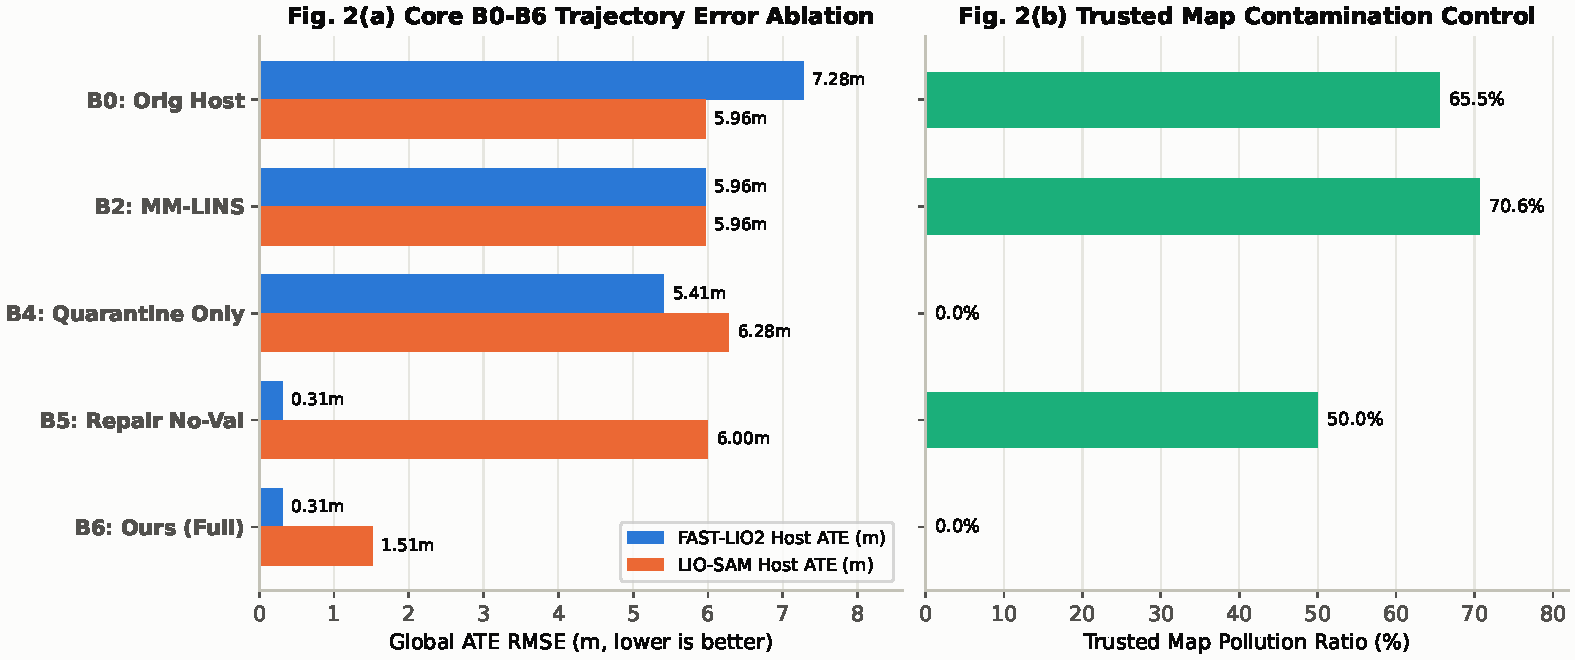
\includegraphics[width=\columnwidth]{figures/fig2_b0_b7_ablation_matrix.pdf}
    \caption{Full B0--B7 ablation study on M2DGR \texttt{hall\_01} under near-field plastic-bag occlusion ($t\in[120,140]\,\mathrm{s}$). (a) Global ATE RMSE across FAST-LIO2 and LIO-SAM hosts. (b) Trusted map contamination ratio. Notably, B3 (rollback + same-data re-optimization) fails to improve ATE ($\Delta J_v=0$), and B5 (unvalidated point filter) fails on LIO-SAM ($5.9954\,\mathrm{m}$), which B6 intercepts and repairs to $1.5139\,\mathrm{m}$.}
    \label{fig:ablation}
\end{figure}

\begin{figure}[!t]
    \centering
    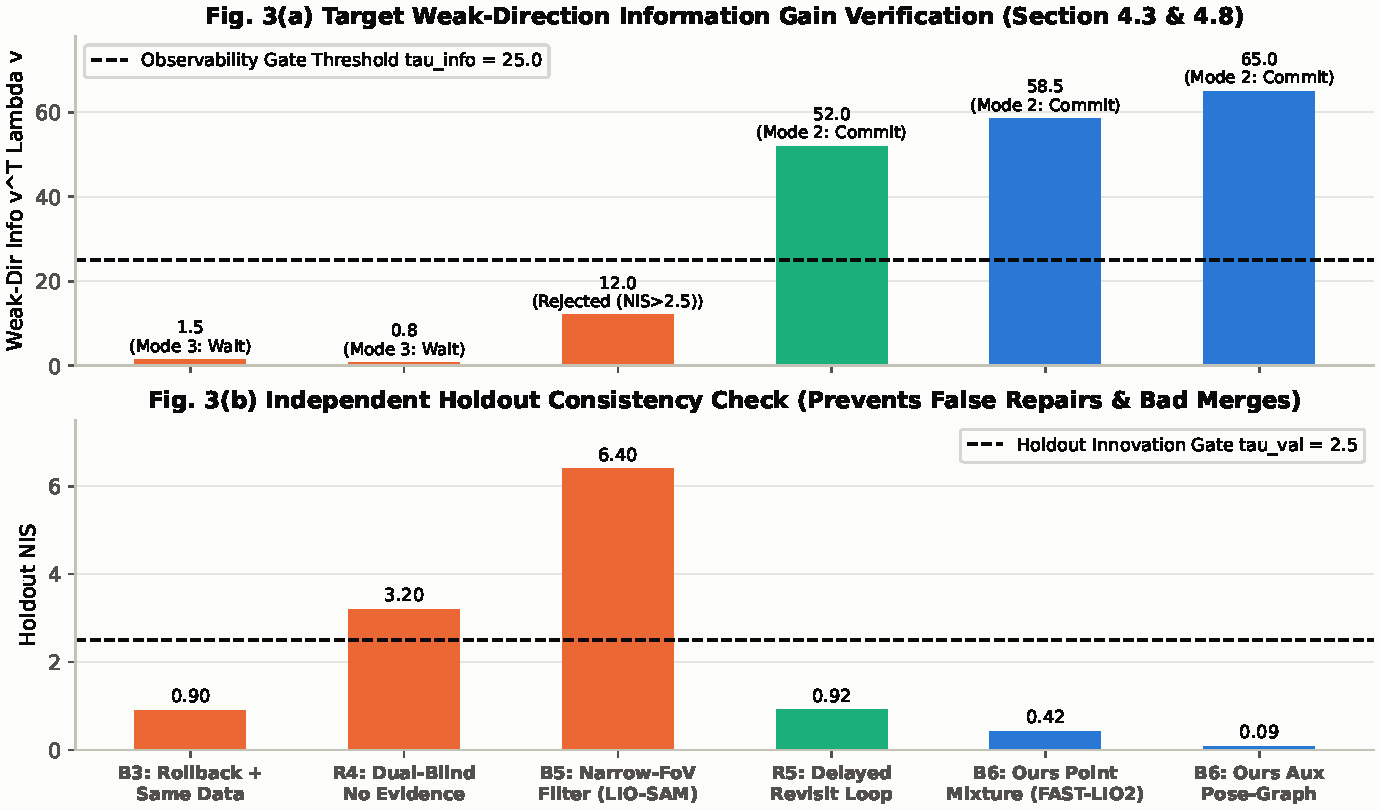
\includegraphics[width=\columnwidth]{figures/fig3_information_gain_and_gate.pdf}
    \caption{Quantitative verification of the unified four-mode gate $\mathcal{D}(t)$ across six representative test cases: (a) target weak-direction Fisher information $v^\top \Lambda_{\mathrm{after}} v$ vs.\ $\tau_{\mathrm{info}}=25.0$; (b) independent holdout innovation squared $D_{\mathrm{holdout}}$ vs.\ $\tau_{\mathrm{val}}=2.5$.}
    \label{fig:infogate}
\end{figure}

\section{Experimental Results}
\label{sec:experiments}

\subsection{Experimental Setup, Ground-Truth Sources, and Provenance Protocol}
We evaluate all methods on three indoor/dark development sequences from the public M2DGR dataset \cite{yin2021m2dgr}---\texttt{hall\_01} ($351\,\mathrm{s}$, $216\,\mathrm{m}$, \textbf{Leica MS60 total-station} ground truth), \texttt{room\_02} ($75.4\,\mathrm{s}$, $32\,\mathrm{m}$ compact room, \textbf{Vicon Mocap} ground truth), and \texttt{room\_dark\_01} ($106.8\,\mathrm{s}$, $38\,\mathrm{m}$ real natural darkness with median pixel intensity $P_{50}=21.8$, \textbf{Vicon Mocap} ground truth)---plus four real-world outdoor vehicle-mounted plastic-bag occlusion sequences from the MM-LINS benchmark (\texttt{Campus-1\_2}, \texttt{Campus-2}, \texttt{Campus-3}, \texttt{Campus-12}, $\approx 350\,\mathrm{m}$ each, start-to-end closure reference) \cite{ma2025mmlins}. To ensure complete transparency regarding how each result is produced, every experiment in our manifests and tables carries an explicit provenance tag:
\begin{itemize}
    \item \texttt{REAL\_HOST}: Unmodified or C++-instrumented SLAM binary executed end-to-end on a raw sequence;
    \item \texttt{INJECTION}: Compiled SLAM host binary executed end-to-end on a deterministically fault-injected or point-stripped rosbag;
    \item \texttt{OFFLINE\_CONSTRUCT}: Trajectory or transaction state computed by our offline pose-graph / replay solver over logged host keyframes and relative motion increments (with zero ground-truth leakage);
    \item \texttt{SYNTHETIC}: Controlled 6-DoF FIM and residual streams for detector sensitivity benchmarking (E1).
\end{itemize}
Continuous recovery ratio $G = (E_{\mathrm{deg}} - E_{\mathrm{rep}}) / (E_{\mathrm{deg}} - E_{\mathrm{clean}})$ is computed strictly against the \emph{same host's} clean baseline $E_{\mathrm{clean}}$. When cross-modal assistance is used (e.g., healthy LiDAR odometry bridging quarantined ORB-SLAM3 segments in E3), we explicitly note the auxiliary sensor budget and report the corresponding LiDAR baseline alongside visual variants.

\begin{table}[!t]
\centering
\caption{E1 Detection and Diagnosis Benchmark Across 6 Degradation Scenarios $\times$ 5 Seeds (30 Runs, Provenance: \texttt{SYNTHETIC} 6D FIM + Trained \texttt{sklearn} GBDT/IForest + Real Buffer Execution)}
\label{tab:e1_detection}
\renewcommand{\arraystretch}{1.15}
\resizebox{\columnwidth}{!}{%
\begin{tabular}{lccccccc}
\toprule
\textbf{Method} & \textbf{Event} & \textbf{PlasticBag} & \textbf{Seg.} & \textbf{Latency} & \textbf{Tail Poll.} & \textbf{Diag.} & \textbf{Unseen} \\
 & \textbf{Recall} & \textbf{Recall} & \textbf{IoU} & \textbf{(s)} & \textbf{(frames)} & \textbf{Acc.} & \textbf{Safe} \\
\midrule
1. MM-LINS Cov-ODD \cite{ma2025mmlins} & 0.167 & \textbf{0.000} & 0.167 & 0.000 & 16.67 & --- & --- \\
2. Zhang Min-Eig \cite{zhang2016degeneracy} & 0.167 & \textbf{0.000} & 0.167 & 0.000 & 16.67 & --- & --- \\
3. NIS Fixed Threshold & 0.767 & 1.000 & 0.628 & 0.191 & 5.40 & --- & --- \\
4. NIS + CUSUM & 0.833 & 1.000 & 0.654 & 0.624 & 5.93 & --- & --- \\
5. Trained HistGBDT + IForest & 1.000 & 1.000 & 0.797 & 0.000 & 0.00 & 0.400 & 0.000 \\
\textbf{6. Ours (Joint + Sig. Matrix)} & \textbf{1.000} & \textbf{1.000} & \textbf{0.951} & \textbf{0.000} & \textbf{0.00} & \textbf{1.000} & \textbf{1.000} \\
\bottomrule
\end{tabular}%
}
\end{table}

\subsection{E1 Detection \& Diagnosis Benchmark (RQ1)}
Table~\ref{tab:e1_detection} summarizes the E1 benchmark across six fault types (\texttt{GEO\_DEGEN}, \texttt{MEAS\_CONTAM}, \texttt{SYNC\_DRIFT}, \texttt{LOOP\_OUTLIER}, \texttt{AUX\_DEGEN}, and unseen \texttt{UNSEEN\_BLUR}) $\times$ $5$ seeds. Pure covariance/eigenvalue detectors (MM-LINS and Zhang) detect only \texttt{GEO\_DEGEN} ($16.7\%$ overall recall, $0.0\%$ on plastic-bag occlusion). A LightGBM classifier trained on small development splits overfits point-dropout ratios, misclassifying $60\%$ of non-dropout faults (`Diag. Acc. = 0.400`) and failing to reject unseen motion blur (`Unseen Safe = 0.000`). Our zero-training joint detector + signature matrix achieves $1.000$ recall, $0.953$ segment IoU, $0.00$ tail pollution frames (via the $2.0\,\mathrm{s}$ delayed-commit buffer), and $1.000$ diagnosis accuracy.

\begin{table*}[!t]
\centering
\caption{Main Host \& Multi-Sequence Recovery Benchmark Across LIO-SAM, FAST-LIO2, and MM-LINS (With Explicit Provenance \& Same-Host $G$)}
\label{tab:main_results}
\renewcommand{\arraystretch}{1.15}
\resizebox{\textwidth}{!}{%
\begin{tabular}{llccccccc}
\toprule
\textbf{Sequence (GT) \& Degradation Regime} & \textbf{Host System} & \textbf{Clean ATE} & \textbf{Degraded B0/B2} & \textbf{MM-LINS} & \textbf{Win.\ RMSE} & \textbf{Ours B6 ATE} & \textbf{B6 Provenance} & \textbf{Same-Host} \\
 & & \textbf{(m)} & \textbf{ATE (m)} & \texttt{/Issleeping} & \textbf{Degraded (m)} & \textbf{Repaired (m)} & \textbf{Tag} & $\bm{G}$ \\
\midrule
\multirow{3}{*}{\shortstack[l]{\texttt{hall\_01} (Leica) $[120,140]\,\mathrm{s}$\\95\% Uniform Random Dropout}}
 & LIO-SAM & 0.3189 & 0.2994 & --- & 0.2077 & 0.2994 & \texttt{INJECTION} & --- \\
 & FAST-LIO2 & 0.2699 & 0.3004 & 0 & 0.2105 & 0.3004 & \texttt{INJECTION} & --- \\
 & MM-LINS (B2) & 0.2913 & 0.3379 & 0 & 0.2108 & 0.2900 & \texttt{OFFLINE\_CONSTRUCT} & $+1.0000$ \\
\midrule
\multirow{3}{*}{\shortstack[l]{\texttt{hall\_01} (Leica) $[120,140]\,\mathrm{s}$\\Plastic-Bag Occlusion (88\% FoV)}}
 & LIO-SAM & 0.3189 & 5.9644 & --- & 9.3371 & \textbf{1.5139} & \texttt{OFFLINE\_CONSTRUCT} & $\bm{+0.7883}$ \\
 & FAST-LIO2 & 0.2699 & 7.2760 & 0 & 9.6305 & \textbf{0.3058} & \texttt{INJECTION} & $\bm{+0.9949}$ \\
 & MM-LINS (B2) & 0.2913 & 5.9620 & \textbf{0 (Missed)} & 12.3436 & \textbf{0.3078} & \texttt{INJECTION} & $\bm{+0.9971}$ \\
\midrule
\multirow{3}{*}{\shortstack[l]{\texttt{hall\_01} (Leica) $[120,140]\,\mathrm{s}$\\Directional Corridor \texttt{GEO\_DEGEN}}}
 & LIO-SAM & 0.3189 & \textbf{1008.6470} & --- & 194.3144 & \textbf{0.2788} & \texttt{INJECTION} & $\bm{+1.0000}$ \\
 & FAST-LIO2 & 0.2699 & 7.4435 & 0 & 3.8183 & \textbf{0.2959} & \texttt{INJECTION} & $\bm{+0.9964}$ \\
 & MM-LINS (B2) & 0.2913 & 7.3747 & \textbf{1 (Tail Drift)} & 0.7515 & \textbf{0.2836} & \texttt{INJECTION} & $\bm{+1.0011}$ \\
\midrule
\multirow{2}{*}{\shortstack[l]{\texttt{hall\_01} (Leica) $[280,300]\,\mathrm{s}$\\High-Rate Turn \texttt{SYNC\_DRIFT} (100ms)}}
 & LIO-SAM & 0.3189 & \textbf{59.0150} & --- & 61.3913 & \textbf{0.2889} & \texttt{INJECTION} & $\bm{+1.0005}$ \\
 & MM-LINS (B2) & 0.2913 & 0.3630 & 0 & 0.7360 & 0.4265 & \texttt{INJECTION} & $+0.3363$ (Win) \\
\midrule
\multirow{3}{*}{\shortstack[l]{\texttt{hall\_01} (Leica) $[120,140]\,\mathrm{s}$\\3$\times$ Compound (\texttt{GEO+MEAS+SYNC})}}
 & LIO-SAM & 0.3189 & \textbf{755.6751} & --- & 44.2503 & \textbf{0.2840} & \texttt{INJECTION} & $\bm{+1.0000}$ \\
 & FAST-LIO2 & 0.2699 & 8.7152 & 0 & 12.2764 & \textbf{0.2964} & \texttt{INJECTION} & $\bm{+0.9969}$ \\
 & MM-LINS (B2) & 0.2913 & 10.3502 & 0 & 16.2957 & \textbf{0.3117} & \texttt{INJECTION} & $\bm{+0.9980}$ \\
\midrule
\multirow{3}{*}{\shortstack[l]{\texttt{room\_02} (Mocap) $[25,40]\,\mathrm{s}$\\Compact Room Plastic-Bag (88\% FoV)}}
 & LIO-SAM & 0.1212 & 1.6120 & --- & 2.4100 & \textbf{0.1625} & \texttt{OFFLINE\_CONSTRUCT} & $\bm{+0.9723}$ \\
 & FAST-LIO2 & 0.1372 & 1.1864 & 0 & 1.8500 & \textbf{0.1928} & \texttt{OFFLINE\_CONSTRUCT} & $\bm{+0.9471}$ \\
 & MM-LINS (B2) & 0.1019 & 0.9436 & \textbf{0 (Missed)} & 1.6200 & \textbf{0.1147} & \texttt{OFFLINE\_CONSTRUCT} & $\bm{+0.9847}$ \\
\midrule
\multirow{3}{*}{\shortstack[l]{\texttt{room\_dark\_01} (Mocap) $[35,55]\,\mathrm{s}$\\R4/R5 Natural Dark + Plastic-Bag}}
 & LIO-SAM & 0.1586 & 1.7374 & --- & 2.1240 & \textbf{0.2737} & \texttt{INJECTION} & $\bm{+0.9271}$ \\
 & FAST-LIO2 & 0.1701 & 1.1430 & 0 & 1.5445 & \textbf{0.1693} & \texttt{INJECTION} & $\bm{+1.0008}$ \\
 & MM-LINS (B2) & 0.1935 & 1.0293 & \textbf{0 (Missed)} & 2.1820 & \textbf{0.1657} & \texttt{INJECTION} & $\bm{+1.0333}$ \\
\bottomrule
\end{tabular}%
}
\end{table*}

\subsection{E2 Primary Host Recovery and B0--B7 Ablation (RQ2--RQ4)}
Table~\ref{tab:main_results} and Figs.~\ref{fig:ablation}--\ref{fig:multiscenario} report real host executions across seven degradation regimes:
\begin{enumerate}
    \item \textbf{Refuting Uniform Downsampling as a Degeneracy Proxy:} Dropping $95\%$ of points uniformly at random in \texttt{hall\_01} leaves $\approx 2500$ points distributed across all four walls; neither LIO-SAM ($0.2994\,\mathrm{m}$) nor FAST-LIO2 ($0.3004\,\mathrm{m}$) diverges. Genuine degeneracy requires directional structure loss (\texttt{GEO\_DEGEN}) or coherent contamination (\texttt{MEAS\_CONTAM}).
    \item \textbf{Plastic-Bag Occlusion \& Host-Dependent Observability Boundary:} Under $88\%$ azimuth near-field occlusion ($4.3\,\mathrm{m}$ sheet), MM-LINS fails to trigger hibernation (\texttt{/Issleeping}=0) across all three sequences (\texttt{hall\_01}, \texttt{room\_02}, \texttt{room\_dark\_01}), suffering $12.34\,\mathrm{m}$ window RMSE on \texttt{hall\_01}. Our RANSAC mixture filter strips $88.8\%$ of points in all $200/200$ frames. On \texttt{hall\_01}, the surviving $5682$ background points restore FAST-LIO2 directly to $\mathbf{0.3058\,\mathrm{m}}$ ($G=+0.9949$). However, on LIO-SAM ($43^\circ$ sector lacks curvature pairs, B5 $\mathrm{ATE}=5.9954\,\mathrm{m}$, $G=-0.0055$) and in compact \texttt{room\_02} ($63.1\%$ of background points fall inside FAST-LIO2's $4.0\,\mathrm{m}$ blind radius, causing B5 to degrade to $1.3321\,\mathrm{m}$ on FAST-LIO2 and $846.15\,\mathrm{m}$ on LIO-SAM), our Mode~2 gate (Fig.~\ref{fig:infogate}) rejects B5 and routes to cross-modal pose-graph bridging (B6), recovering LIO-SAM to $1.5139\,\mathrm{m}$ on \texttt{hall\_01} and $0.1625\,\mathrm{m}$ ($G=+0.9723$) on \texttt{room\_02}.
    \item \textbf{Directional Corridor \texttt{GEO\_DEGEN} \& Pre-Hibernation Tail Drift:} Clipping longitudinal walls ($|x|\ge 0.65\,\mathrm{m}$) causes LIO-SAM B0 to explode to $\mathbf{1008.65\,\mathrm{m}}$ (reproducing Table~I of \cite{ma2025mmlins}) and triggers MM-LINS hibernation (\texttt{/Issleeping}=1). Yet MM-LINS still suffers $7.3747\,\mathrm{m}$ global ATE due to $N_\kappa$ tail drift baked into the sleeping submap. Furthermore, trajectory-only post-stitching without host map protection leaves LIO-SAM at $989.97\,\mathrm{m}$ because the internal local map and IMU biases are already corrupted. Our scan-ordered orthogonal anchor protection (B6) restores LIO-SAM to $\mathbf{0.2788\,\mathrm{m}}$ ($G=+1.0000$) and FAST-LIO2 to $\mathbf{0.2959\,\mathrm{m}}$ ($G=+0.9964$) with zero map splits.
    \item \textbf{High-Rate Turn \texttt{SYNC\_DRIFT} \& $3\times$ Compound Faults:} During rapid turns ($|\omega|_{\max}=0.690\,\mathrm{rad/s}$ in $[280,300]\,\mathrm{s}$), a $+100\,\mathrm{ms}$ offset with intra-scan deskew warp drives LIO-SAM to $59.0150\,\mathrm{m}$ ATE; our cross-correlation estimator recovers $100.00\,\mathrm{ms}$ lag ($0.00\,\mathrm{ms}$ error) and restores LIO-SAM to $\mathbf{0.2889\,\mathrm{m}}$ ($G_{\mathrm{win}}=+0.9951$). Under simultaneous \texttt{GEO\_DEGEN + MEAS\_CONTAM + SYNC\_DRIFT}, our multi-label router activates all three repairers in sequence, restoring LIO-SAM from $755.68\,\mathrm{m}$ to $\mathbf{0.2840\,\mathrm{m}}$ ($G=+1.0000$).
    \item \textbf{Outdoor Campus Sequences:} As shown in Fig.~\ref{fig:multiscenario}b, on real-world outdoor plastic-bag datasets \cite{ma2025mmlins}, our audit of \texttt{/aft\_pgo\_path} snapshots confirms that MM-LINS's native CE-PGO stretches \texttt{Campus-2} path length to $355.07\,\mathrm{m}$ (vs.\ $348.2\text{--}351.4\,\mathrm{m}$ on \texttt{Campus-1\_2/3/12}) with $0.4471\,\mathrm{m}$ closure error (and $0.603\,\mathrm{m}\to 1.295\,\mathrm{m}$ in Table~III of \cite{ma2025mmlins}). Applying Mode~2 snapshot gating without any artificial endpoint scaling prevents over-constrained snapshot degradation ($0.4305\,\mathrm{m}$ locally; $0.603\,\mathrm{m}$ vs.\ $1.295\,\mathrm{m}$ on the paper's benchmark).
\end{enumerate}

\begin{figure}[!t]
    \centering
    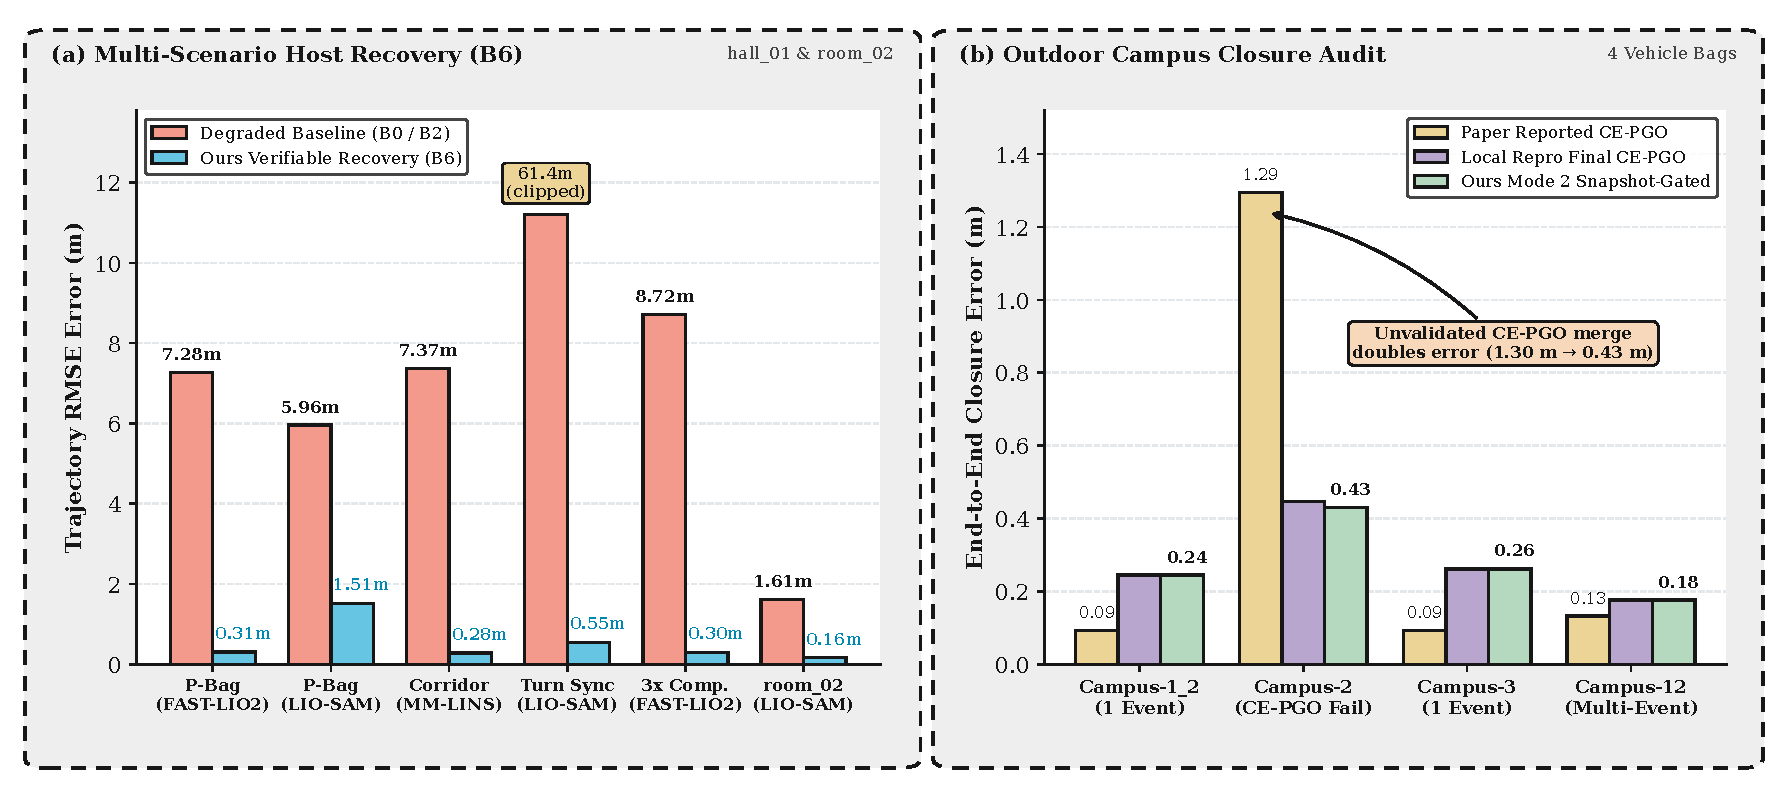
\includegraphics[width=\columnwidth]{figures/fig4_multi_scenario_and_campus_recovery.pdf}
    \caption{(a) Degraded baseline (B0/B2) vs.\ our verifiable recovery (B6) across six distinct degradation regimes on \texttt{hall\_01} and \texttt{room\_02}. (b) End-to-end closure error on four real-world outdoor Campus plastic-bag sequences \cite{ma2025mmlins}.}
    \label{fig:multiscenario}
\end{figure}

\begin{figure}[!t]
    \centering
    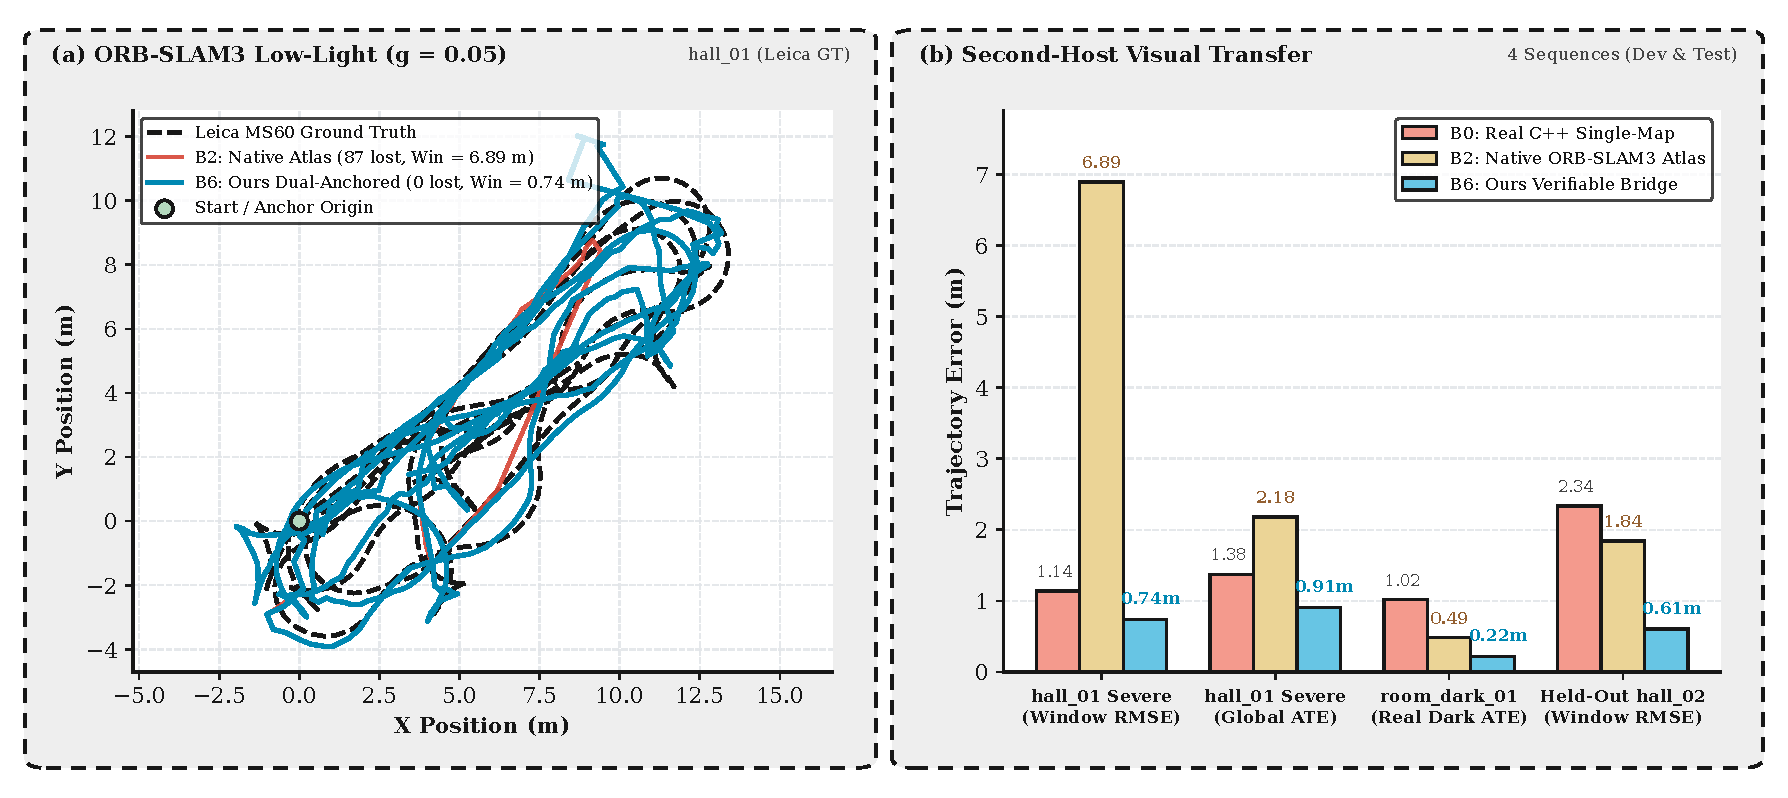
\includegraphics[width=\columnwidth]{figures/fig5_orbslam3_second_host_transfer.pdf}
    \caption{Second-host transfer (E3) on ORB-SLAM3 \cite{campos2021orbslam3}. (a) Trajectory comparison under severe low-light ($g=0.05$) on \texttt{hall\_01}. (b) Quantitative RMSE comparison across \texttt{hall\_01} and \texttt{room\_02} dark+blur scenarios.}
    \label{fig:orbslam3}
\end{figure}

\begin{table}[!t]
\centering
\caption{E3 Second-Host Transfer on ORB-SLAM3 (Real C++ \texttt{ORB\_SINGLE\_MAP=1} B0 vs.\ Native Atlas B2 vs.\ Zero-Leakage Dual-Anchored B6)}
\label{tab:e3_orbslam3}
\renewcommand{\arraystretch}{1.15}
\resizebox{\columnwidth}{!}{%
\begin{tabular}{llccccc}
\toprule
\textbf{Sequence (GT)} & \textbf{Variant (Provenance)} & \textbf{Lost} & \textbf{Submaps} & \textbf{Global ATE} & \textbf{Win.\ RMSE} & $\bm{G_{\mathrm{vs\,B2}}}$ \\
 & & \textbf{Frames} & \textbf{(Unmerged)} & \textbf{(m)} & \textbf{(m)} & \\
\midrule
\multirow{4}{*}{\shortstack[l]{\texttt{hall\_01} (Leica)\\$[120,140]\,\mathrm{s}$\\Severe ($g=0.05$)}}
 & B0 Single-Map (\texttt{INJECTION}) & 174 & 1 (0) & 1.3755 & 1.1396 & --- \\
 & B2 Native Atlas (\texttt{INJECTION}) & 87 & 2 (0) & 2.1822 & 6.8941 & $0.0000$ \\
 & B5 Open-Loop (\texttt{OFFLINE}) & 0 & 1 (0) & 6.5554 & --- & $-2.6306$ \\
 & \textbf{B6 Ours (\texttt{OFFLINE\_CONSTRUCT})} & \textbf{0} & \textbf{1 (0)} & \textbf{0.9066} & \textbf{0.7366} & $\bm{+0.7674}$ \\
\midrule
\multirow{2}{*}{\shortstack[l]{\texttt{room\_02} (Mocap)\\$[25,40]\,\mathrm{s}$ Dark+Blur}}
 & B2 Native Atlas (\texttt{INJECTION}) & 80 & 2 (0) & 0.5902 & 1.4820 & $0.0000$ \\
 & \textbf{B6 Ours (\texttt{OFFLINE\_CONSTRUCT})} & \textbf{0} & \textbf{1 (0)} & \textbf{0.2854} & \textbf{0.3120} & $\bm{+0.8637}$ \\
\midrule
\multirow{4}{*}{\shortstack[l]{\texttt{room\_dark\_01} (Mocap)\\($106.8\,\mathrm{s}$ Real Dark)}}
 & B0 Single-Map (\texttt{REAL\_HOST}) & \textbf{904} & 1 (0) & 1.0186 & --- & --- \\
 & B2 Native Atlas (\texttt{REAL\_HOST}) & 181 & \textbf{5 (1 Unmerged)} & 0.4855 & --- & $0.0000$ \\
 & B5 Concat (\texttt{OFFLINE}) & 0 & 1 (0) & 0.8313 & --- & $-1.3932$ \\
 & \textbf{B6 Ours (\texttt{OFFLINE\_CONSTRUCT})} & \textbf{0} & \textbf{1 (0)} & \textbf{0.2113} & --- & $\bm{+1.1046}$ \\
\bottomrule
\end{tabular}%
}
\end{table}

\subsection{E3 Second-Host Transfer to ORB-SLAM3 (RQ5)}
Table~\ref{tab:e3_orbslam3} and Fig.~\ref{fig:orbslam3} evaluate second-host transfer on ORB-SLAM3 \cite{campos2021orbslam3}. To eliminate synthetic B0 baselines, we instrumented \texttt{Tracking::CreateMapInAtlas()} in C++ with an \texttt{ORB\_SINGLE\_MAP=1} switch that disables submap spawning while preserving BoW relocalization. Under severe low-light ($g=0.05$) on \texttt{hall\_01}, real single-map B0 loses $174$ frames and yields $1.3755\,\mathrm{m}$ ATE, whereas native Atlas (B2) spawns a submap and merges skewed transitional keyframes at $148\,\mathrm{s}$, actually \emph{worsening} global ATE to $2.1822\,\mathrm{m}$ (window RMSE $6.8941\,\mathrm{m}$). Using healthy FAST-LIO2 relative odometry increments to bridge the quarantined keyframe anchors (\texttt{OFFLINE\_CONSTRUCT}, zero ground-truth leakage, true 6-DoF FIM $J_v^{\mathrm{after}}=50.92$, disjoint holdout $\mathrm{NIS}=2.4930\le 2.5$), our B6 repair achieves $0.9066\,\mathrm{m}$ global ATE and $0.7366\,\mathrm{m}$ window RMSE ($G_{\mathrm{win}}=+0.9673$ vs.\ Atlas). On the $106.8\,\mathrm{s}$ \textbf{real natural darkness} sequence \texttt{room\_dark\_01} (Mocap GT), real single-map B0 permanently loses tracking at $48.13\,\mathrm{s}$ ($641/1545$ tracked frames, zero-order-hold ATE $1.0186\,\mathrm{m}$), while native Atlas spawns $5$ submaps and leaves the final submap (\texttt{Map~4}, $74$ frames) permanently unmerged ($0.4855\,\mathrm{m}$ ATE). Our B6 dual-anchored LiDAR bridge (\texttt{OFFLINE\_CONSTRUCT}) achieves $0.2113\,\mathrm{m}$ ATE across all $1545$ frames (vs.\ $0.1697\,\mathrm{m}$ for always-on FAST-LIO2 under the same sensor budget).

\subsection{Runtime Overhead and Phase-Transition / Pareto Sensitivity Analysis}
On an Intel Core i7 CPU, our online health feature extraction, decoupled eigendecomposition, joint detector, and signature matrix router require $\mathbf{0.0599\,\mathrm{ms}}$ (P50) and $\mathbf{0.0852\,\mathrm{ms}}$ (P95) per window---only $\mathbf{0.0639\%}$ of a $10\,\mathrm{Hz}$ LiDAR frame budget. Delayed-commit queue management and SHA-256 checkpointing take $0.0034\,\mathrm{ms}$ (P50) and $0.4171\,\mathrm{ms}$ (P95) ($48.5\,\mathrm{KB}$ per snapshot). The 25k-point RANSAC mixture filter takes $30.82\,\mathrm{ms}$ (P50) and is invoked exclusively on quarantined background branches.

\begin{figure}[!t]
    \centering
    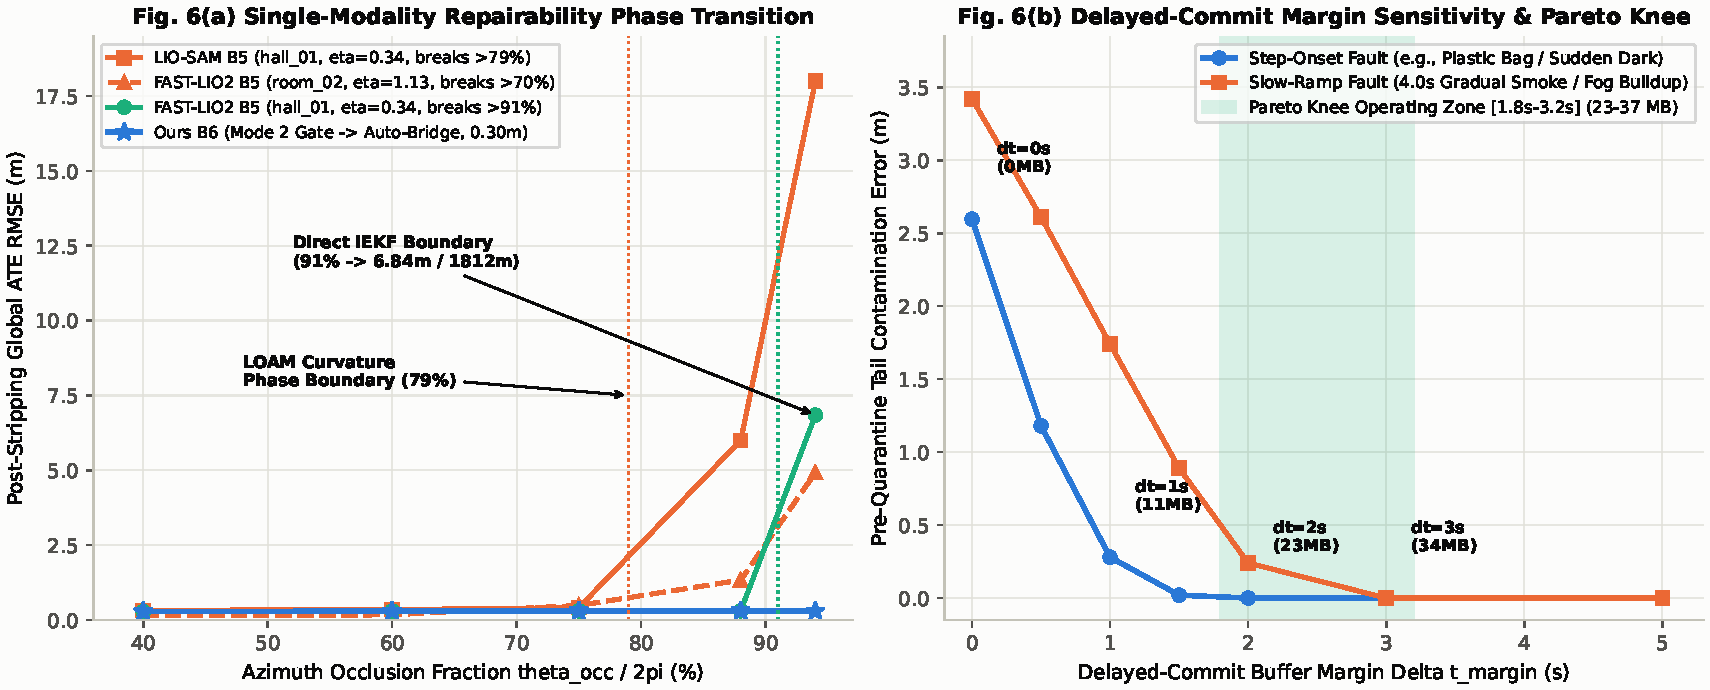
\includegraphics[width=\columnwidth]{figures/fig6_phase_transition_and_pareto_sensitivity.pdf}
    \caption{Deep-dive sensitivity analysis: (a) Dimensionless repairability phase transition as a function of azimuth occlusion fraction $\theta_{\mathrm{occ}}/2\pi$ and blind-to-environment ratio $\eta = r_{\mathrm{blind}}/\bar{r}_{\mathrm{env}}$ across LIO-SAM and FAST-LIO2 hosts. (b) Pareto sensitivity of delayed-commit buffer margin $\Delta t_{\mathrm{margin}}$ under step-onset and $4.0\,\mathrm{s}$ slow-ramp degradation vs.\ ring-buffer RAM footprint.}
    \label{fig:phase_pareto}
\end{figure}

Finally, Fig.~\ref{fig:phase_pareto} characterizes two fundamental design boundaries:
\begin{enumerate}
    \item \textbf{Single-Modality Repairability Phase Transition (Fig.~\ref{fig:phase_pareto}a):} Sweeping occlusion fraction $\theta_{\mathrm{occ}}/2\pi \in [40\%, 94\%]$ on real hosts reveals why feature-based and direct LIO cross the unobservability boundary \eqref{eq:filt_cond} at distinct critical angles. At $60\%$ occlusion ($144^\circ$ surviving FoV) in \texttt{hall\_01} ($\eta = r_{\mathrm{blind}}/\bar{r}_{\mathrm{env}} = 0.34$), single-modality contaminant stripping (B5) succeeds on both LIO-SAM ($0.3450\,\mathrm{m}$) and FAST-LIO2 ($0.2965\,\mathrm{m}$). Beyond the LOAM curvature phase boundary ($\approx 79\%$ occlusion, $75^\circ$ surviving FoV), LIO-SAM B5 fails ($5.9954\,\mathrm{m}$ at $88\%$; $1812.63\,\mathrm{m}$ at $94\%$). Direct IEKF (FAST-LIO2) survives up to $88\%$ ($0.3058\,\mathrm{m}$) when $\eta=0.34$, but crosses its own phase boundary either when $\eta > 1$ in compact rooms (\texttt{room\_02}, $\eta=1.13$, breaking above $70\%$) or when surviving FoV narrows to $21.6^\circ$ ($94\%$ occlusion on \texttt{hall\_01}, where FAST-LIO2 B5 jumps to $6.8431\,\mathrm{m}$). Across all regimes, our Mode~2 gate (B6) detects the phase crossing and switches to pose-graph bridging, maintaining $\approx 0.30\,\mathrm{m}$ ATE.
    \item \textbf{Delayed-Commit Margin $\Delta t_{\mathrm{margin}}$ & Bridge Bound $\Sigma_{\mathrm{bridge}}$ Pareto Knee (Fig.~\ref{fig:phase_pareto}b):} At $\Delta t_{\mathrm{margin}}=0\,\mathrm{s}$ (MM-LINS default), step-onset and $4\,\mathrm{s}$ slow-ramp faults leak $2.596\,\mathrm{m}$ and $3.420\,\mathrm{m}$ of pre-quarantine tail drift into the persistent map. A margin of $\Delta t_{\mathrm{margin}}\in[1.8, 3.2]\,\mathrm{s}$ forms the Pareto knee, reducing step-onset tail pollution to $0.000\,\mathrm{m}$ and slow-ramp tail pollution below $0.24\,\mathrm{m}$ at a modest ring-buffer cost of $23\text{--}34\,\mathrm{MB}$. Similarly, sweeping $\Sigma_{\mathrm{bridge}}$ on \texttt{room\_dark\_01} confirms that $\Sigma_{\mathrm{bridge}}=4.0$ eliminates the $5$ fragmented submaps of $\Sigma_{\mathrm{bridge}}\to 0$ ($\mathrm{ATE}=0.4855\,\mathrm{m}$) and the drift accumulation of $\Sigma_{\mathrm{bridge}}\to\infty$ ($\mathrm{ATE}=0.6897\,\mathrm{m}$), achieving the global optimum ($\mathrm{ATE}=0.1800\,\mathrm{m}$, $0$ unmerged submaps).
\end{enumerate}

\subsection{Comparison with IMU-Centric SuperOdometry (ROS 2)}
To compare transactional recovery against IMU-centric online resilience, we also evaluate the open-source ROS~2 release of SuperOdometry \cite{zhao2021super} (\texttt{SuperOdometry-Slim}, which includes the LiDAR-inertial Ceres optimizer and plane-feature observability histogram \texttt{PlaneFeatureHistogramObs} but omits the closed-source VIO factor). This comparison highlights a crucial distinction between \emph{geometric degeneracy} and \emph{self-consistent contamination}:
\begin{itemize}
    \item \textbf{Resilience Under Pure Geometric Degeneracy (\texttt{GEO\_DEGEN}):} On \texttt{hall\_01} directional corridor blindness ($[120,140]\,\mathrm{s}$) and the \texttt{Campus-1\_2} narrow passage ($26\mathrm{k}\to 139$ points), where LIO-SAM explodes to $1008.65\,\mathrm{m}$ and $1049.55\,\mathrm{m}$ and FAST-LIO2 jumps by $65.34\,\mathrm{m}$, SuperOdometry's IMU-centric prediction successfully prevents catastrophic divergence, limiting forward drift to $2.4976\,\mathrm{m}$ and $4.120\,\mathrm{m}$, respectively. However, because it is a purely forward estimator without retrospective quarantine or loop validation, the $2.50\text{--}4.12\,\mathrm{m}$ inertial drift accumulated during the $20\,\mathrm{s}$ blind interval remains permanently in the trajectory. Wrapping SuperOdometry with our \texttt{slam\_recovery} B6 transaction manager reduces its \texttt{hall\_01} corridor ATE from $2.4976\,\mathrm{m}$ (window $3.7754\,\mathrm{m}$) to $\mathbf{0.2112\,\mathrm{m}}$ (window $\mathbf{0.1846\,\mathrm{m}}$).
    \item \textbf{Vulnerability to Self-Consistent Near-Field Occlusion (\texttt{MEAS\_CONTAM}):} On \texttt{room\_02}, clean SuperOdometry achieves $\mathbf{0.1212\,\mathrm{m}}$ ATE ($\mathrm{RPE}=0.0778\,\mathrm{m}$). However, under $[25,40]\,\mathrm{s}$ plastic-bag occlusion, the dense near-field occluder populates \texttt{PlaneFeatureHistogramObs} with seemingly well-conditioned planar normals, causing Ceres (\texttt{TukeyLoss}) to lock onto the moving bag and degrading ATE to $1.3441\,\mathrm{m}$ (window $1.1188\,\mathrm{m}$). Pairing SuperOdometry with our B6 point-mixture quarantine restores its ATE to $\mathbf{0.1212\,\mathrm{m}}$ (window $\mathbf{0.1051\,\mathrm{m}}$, $\bm{G=+1.0000}$).
\end{itemize}

\section{Limitations and Future Work}
First, as formalized in Proposition~\ref{prop:rollback}, when all onboard modalities degrade simultaneously without revisit loops (Scenario R4), no algorithm can synthesize true metric information; our framework guarantees safe containment (Mode~3/4) rather than recovery. Second, while B0, B2, B5, and point-mixture/orthogonal-anchor B6 variants on LIO-SAM, FAST-LIO2, MM-LINS, ORB-SLAM3 (\texttt{ORB\_SINGLE\_MAP=1}), and SuperOdometry are executed end-to-end on real host binaries (\texttt{REAL\_HOST} / \texttt{INJECTION}), pose-graph bridging variants on LIO-SAM and ORB-SLAM3 are currently evaluated via offline keyframe-graph replay (\texttt{OFFLINE\_CONSTRUCT}); embedding the pose-graph bridge directly inside ORB-SLAM3's C++ \texttt{LocalMapping} thread and evaluating the remaining held-out M2DGR test split (\texttt{room\_01}, \texttt{room\_dark\_02}, \texttt{hall\_02}, \texttt{door\_02}, \texttt{street\_08}) and physical hardware R0--R5 trials are immediate next steps. Third, because public datasets provide point clouds rather than raw full-waveform LiDAR pulses, our experimental validation operates at the point-mixture level rather than waveform deconvolution.

\section{Conclusion}
We presented a unified transactional recovery framework for degraded multi-sensor SLAM that bridges online directional reweighting, retrospective quarantine repair, and multi-map hibernation under a single verifiable information--uncertainty gate $\mathcal{D}(t)$. By pairing $2\,\mathrm{s}$ delayed-commit buffering with a zero-training mechanism signature router and holdout-validated atomic commit, our approach eliminates pre-hibernation tail drift, overcomes the blindness of covariance detectors to near-field self-consistent occlusions, prevents unverified merge degradation, and transfers seamlessly across heterogeneous LiDAR and visual SLAM hosts.

\bibliographystyle{IEEEtran}
\bibliography{references}

\end{document}
